\documentclass{article}
\usepackage{graphicx}
\usepackage{float}
\usepackage[spanish]{babel}
\usepackage{hyperref}
\usepackage{csquotes}
\graphicspath{ {img/} }
\setlength{\parskip}{\baselineskip}

\title{Areas Recreativas - Sprint 1 \\[3ex] \small PAMN - Programación de Aplicaciónes Moviles Nativas}

\author{Chamil José Cruz Razeq}

\begin{document}
    \maketitle
    \thispagestyle{empty}
    \newpage

    \section{Introducción}
        Todos los informes sobre las tareas propuestas se encuentran disponibles en el
         siguiente repositorio de \href{https://github.com/chamilstudy/ulpgc_pamn_labs}{GitHub}
         y la aplicación se encuentra en \href{https://github.com/chamilstudy/pamn_proyecto_final}{GitHub}.

        Este documento recoge la información referente al primer sprint del desarrollo de la
         aplicación de Areas Recreativas.
    
    \section{Historias de Usuario}

    Entre las historias de usuario planteadas, se han seleccionado para el primer sprint:
    
    \begin{figure}[H]
        \centerline{\includegraphics[scale=0.4]{historias.png}}
        \caption{Historias de usuario}
        \label{fig:historias}
    \end{figure}

    Donde podemos establecer los siguientes objetivos:

    \begin{itemize}
        \item Definir la navegación y distintas pantallas:
        \begin{enumerate}
            \item Login
            \item Registro
            \item Principal
            \item Reservas
            \item Emergencias
            \item Perfil
        \end{enumerate}
        \item Crear las pantallas de Login y Registro, sus modelos y conexión con Firebase.
        \item Definir colores y tema, además de la distinción entre modo claro y oscuro.
        \item Crear la barra de navegación y la lógica de navegación.
    \end{itemize}

    \section{Estimación en tiempo de cada historia}

    Podríamos agrupar las historias en:

    \begin{enumerate}
        \item Barra y lógica de navegación, temas y colores podrían completarse en 8 horas.
        \item Login y registro se podrían completar en unas 6 horas.
    \end{enumerate}

    Adicionalmente, al tratarse del primer sprint, configurar el proyecto, crear directorios y
     ficheros, configurar el manifiesto y ficheros de build podría llevar unas 4 horas.

    \section{Reparto de tareas}

    Todas las tareas serán desarrolladas por el autor de este documento.

    \section{Muestra de desarrollo}
    
    \begin{figure}[H]
        \centerline{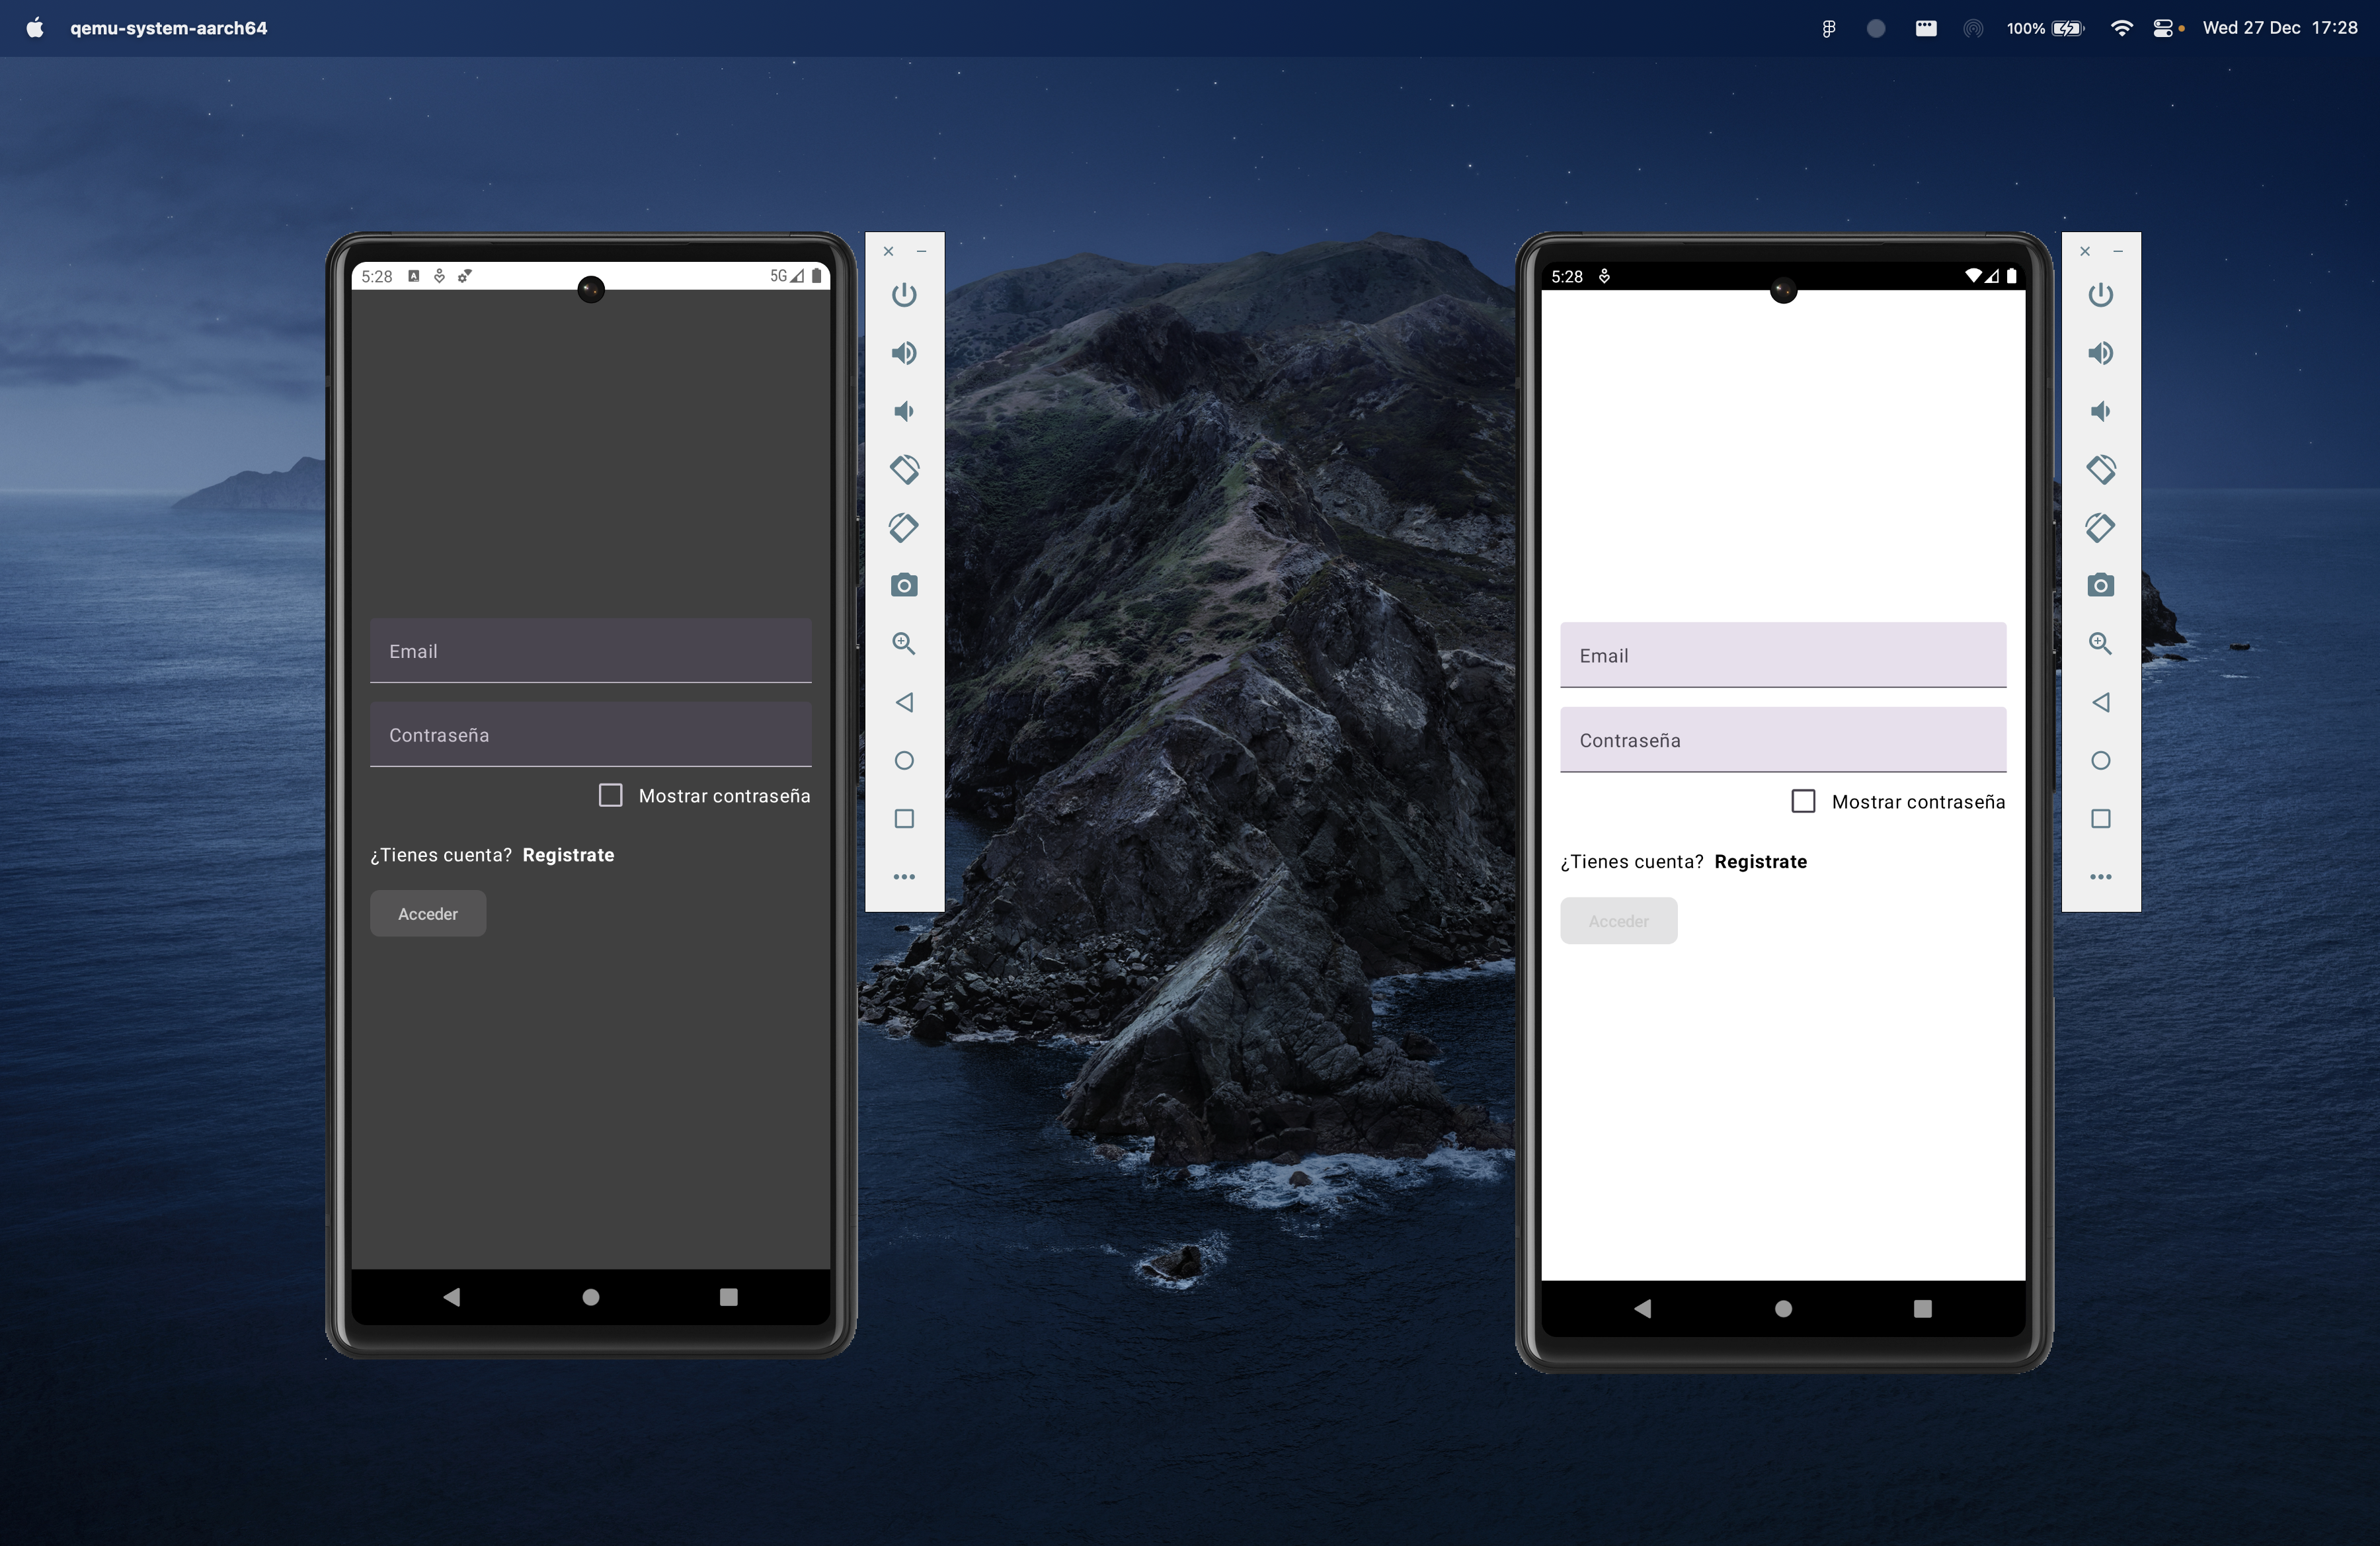
\includegraphics[scale=0.2]{login.png}}
        \caption{Pantalla de login}
        \label{fig:login}
    \end{figure}

    \begin{figure}[H]
        \centerline{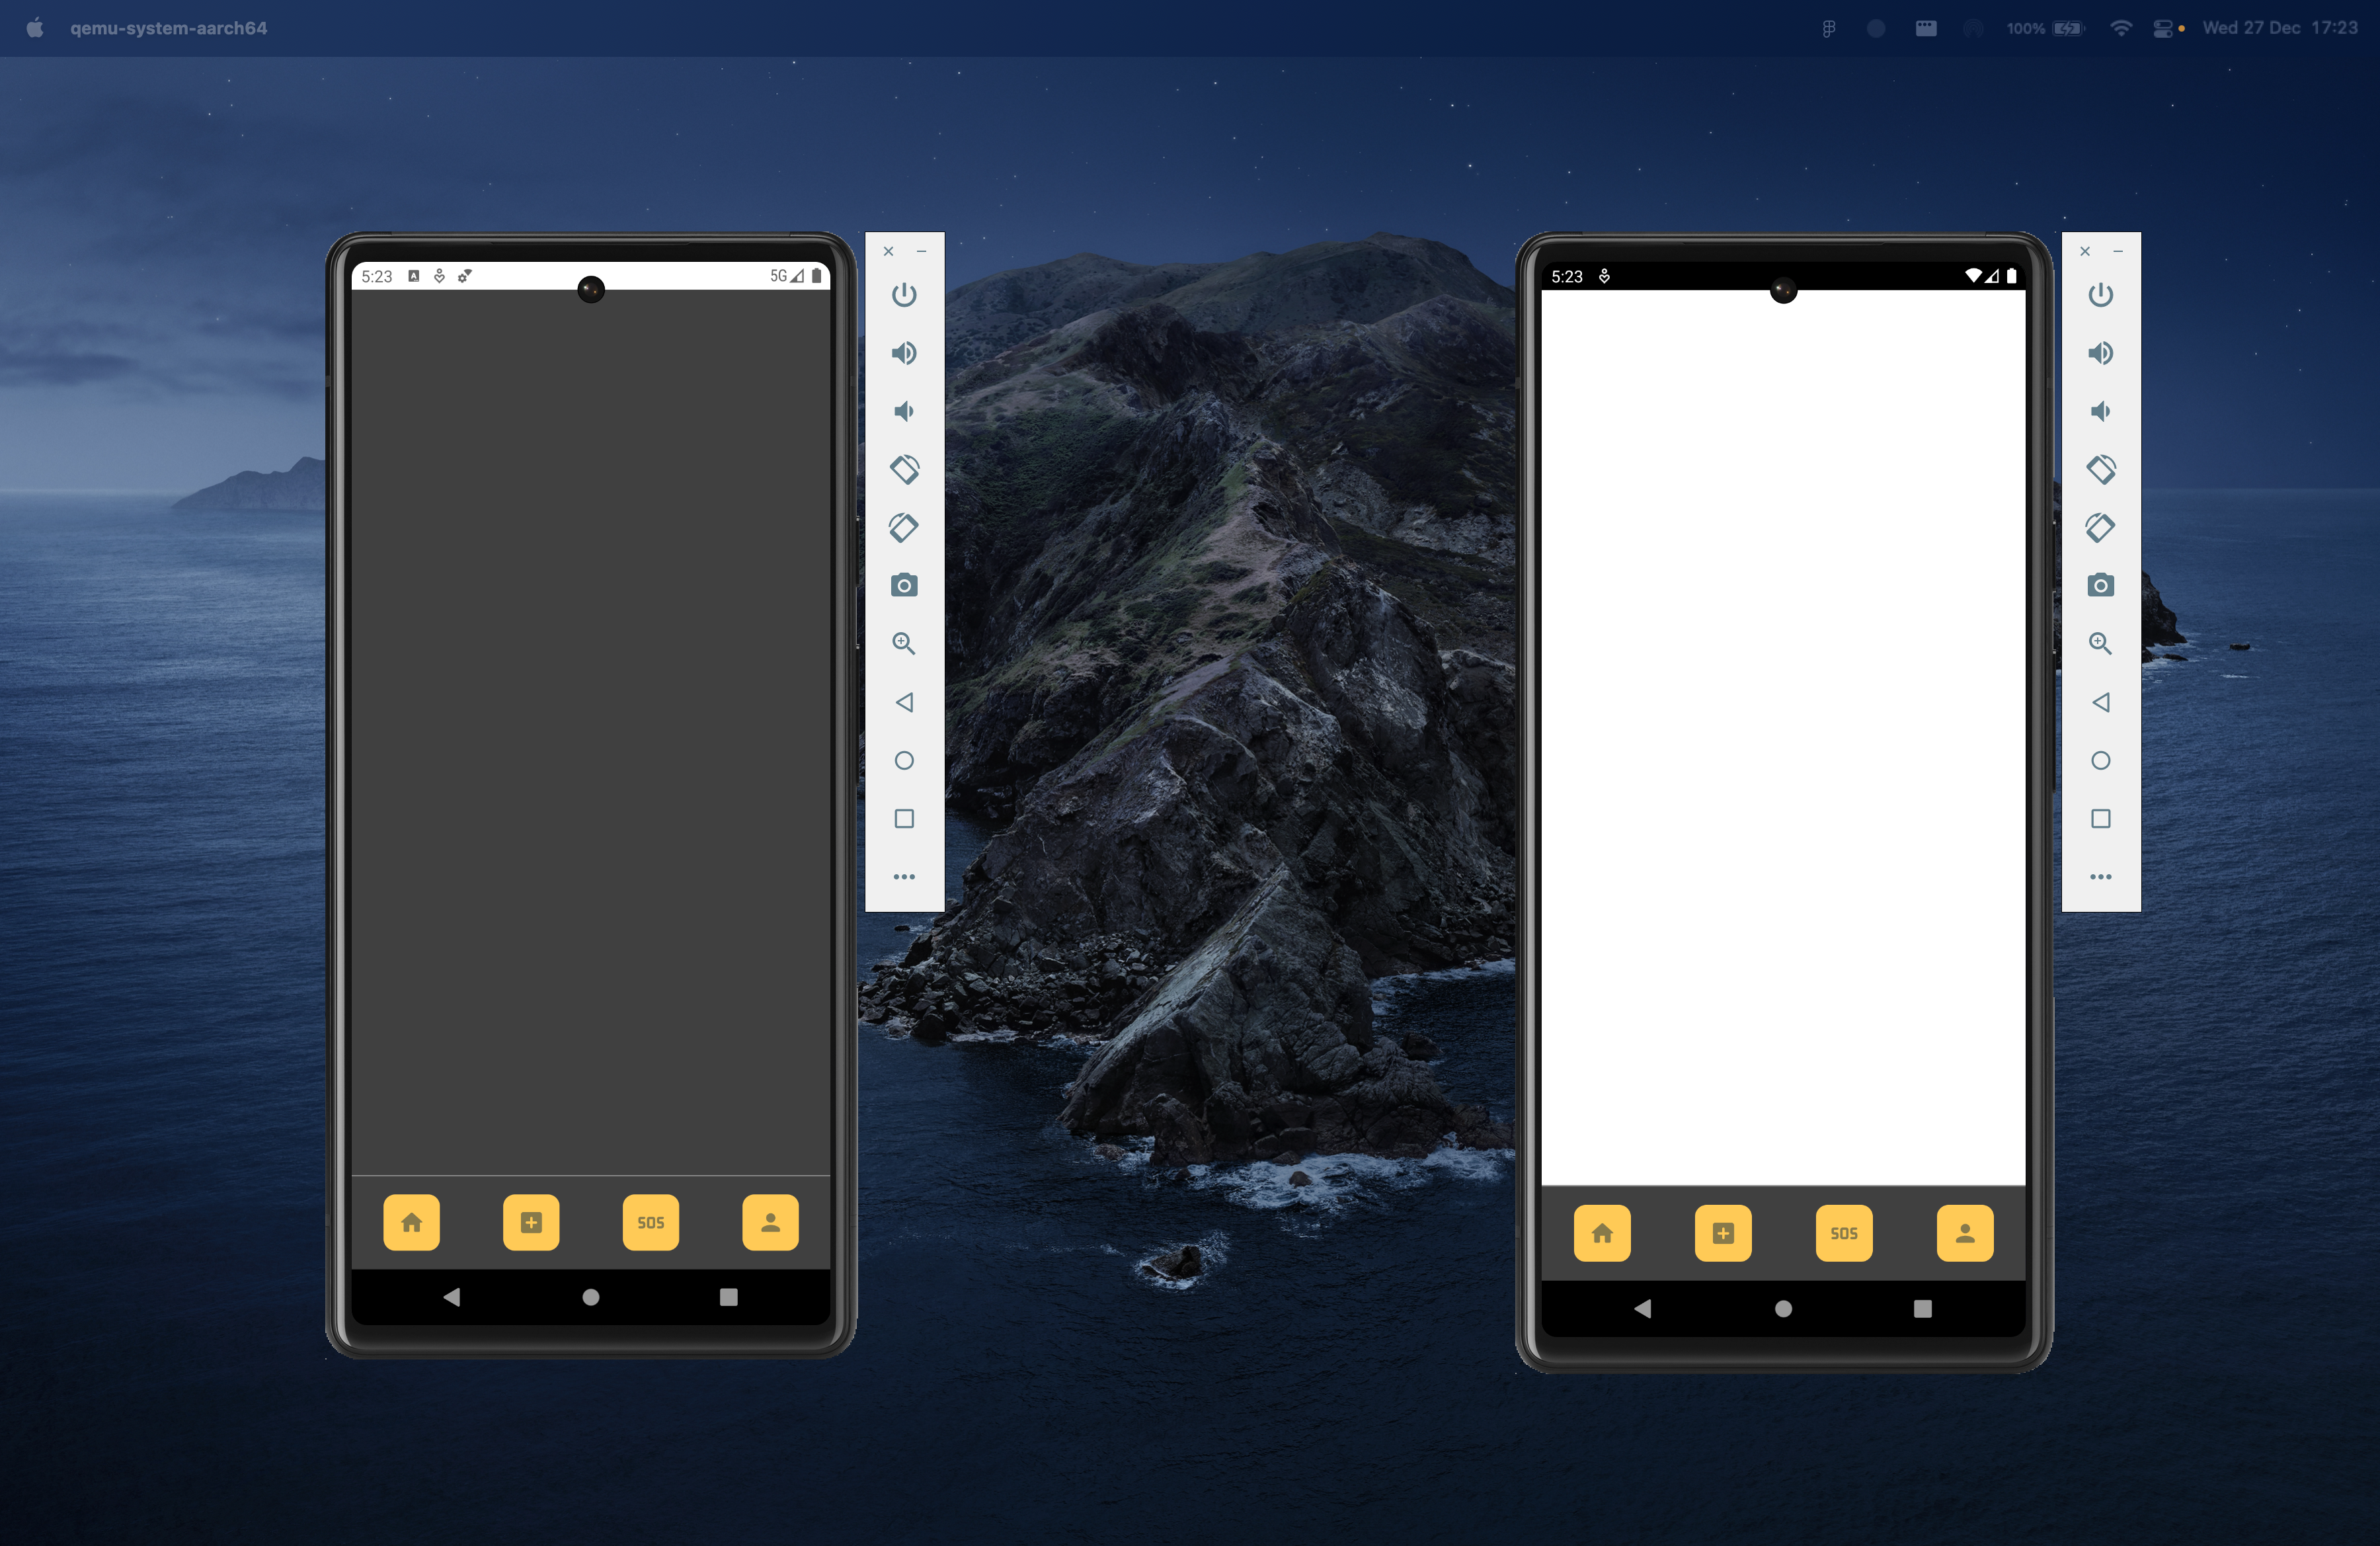
\includegraphics[scale=0.2]{home.png}}
        \caption{Cuálquier pantalla con la barra de navegación}
        \label{fig:home}
    \end{figure}
\end{document}